% Layout fixture: one-column lecture notes (article class, Computer Modern).
% Written for a11y-stem's tests; no third-party text. Build: make_pdfs.py in this folder.
\documentclass[11pt]{article}
% Computer Modern text fonts (CMR, CMBX), as pdfLaTeX writes them; XeTeX defaults to Latin Modern.
\usepackage[OT1]{fontenc}
\renewcommand{\rmdefault}{cmr}
\usepackage{amsmath,amssymb}
\usepackage{tikz}
\usepackage[margin=1in]{geometry}
\pagestyle{plain}

\begin{document}

\section{Derivatives}

The derivative of a function $f$ at a point $a$ measures how quickly $f(x)$ changes
when $x$ is close to $a$. It is defined as the limit
\begin{equation}
  f'(a) = \lim_{h \to 0} \frac{f(a+h) - f(a)}{h}
  \label{eq:definition}
\end{equation}
whenever that limit exists. A function with a derivative at every point of an interval
is called differentiable there, and its graph has no corners on that interval.

\subsection{Rules for derivatives}

Three rules cover most of the functions met in this course:
\begin{itemize}
  \item the power rule, $\frac{d}{dx} x^n = n x^{n-1}$ for every real $n$;
  \item the product rule, which also works
  \begin{itemize}
    \item for three factors at once, and
    \item for any number of factors by induction;
  \end{itemize}
  \item the chain rule for compositions.
\end{itemize}
Written out in full, the product and chain rules read
\begin{align}
  \frac{d}{dx}\bigl(u v\bigr) &= u' v + u v', \label{eq:product}\\
  \frac{d}{dx} f\bigl(g(x)\bigr) &= f'\bigl(g(x)\bigr)\, g'(x). \label{eq:chain}
\end{align}

\section{Integrals}

\subsection{The fundamental theorem}

If $F$ is an antiderivative of a continuous function $f$ on $[a, b]$, so that
$F' = f$, then
\[
  \int_a^b f(x)\,dx = F(b) - F(a).
\]
A Riemann sum with $n$ strips of width $\Delta x$ approximates the same area:
\begin{equation}
  \sum_{i=1}^{n} f(x_i)\,\Delta x \approx \int_a^b f(x)\,dx .
  \label{eq:riemann}
\end{equation}

\subsection{Exercises}

\begin{enumerate}
  \item Compute $\int_0^1 x^2\,dx$ with the fundamental theorem.
  \item Show that
  \begin{enumerate}
    \item $\int_0^{\pi} \sin x\,dx = 2$, and
    \item the area under $y = e^x$ between $x = 0$ and $x = 1$ is $e - 1$.
  \end{enumerate}
  \item Estimate the integral in the first exercise with four strips.
\end{enumerate}

\begin{figure}[h]
  \centering
  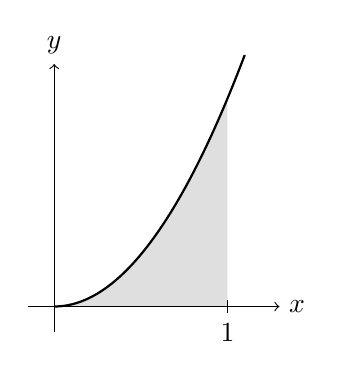
\begin{tikzpicture}[scale=1.1]
    \fill[gray!25] (0,0) -- plot[domain=0:2, samples=40] (\x, {0.6*\x*\x}) -- (2,0) -- cycle;
    \draw[->] (-0.3,0) -- (2.6,0) node[right] {$x$};
    \draw[->] (0,-0.3) -- (0,2.8) node[above] {$y$};
    \draw[thick, domain=0:2.2, samples=50] plot (\x, {0.6*\x*\x});
    \draw (2,0.08) -- (2,-0.08) node[below] {$1$};
  \end{tikzpicture}
  \caption{The area under $y = x^2$ between $x = 0$ and $x = 1$.}
  \label{fig:area}
\end{figure}

\end{document}
